\chapter{Integral Probability Metrics}
\label{ch:ipm}

\section{Distances Between Distributions: Beyond Pointwise Comparison}

In the study of deep learning and information theory, we frequently encounter the need to measure the discrepancy between two probability distributions. Whether we are training a generative model to match a data distribution, or bounding the generalization gap of a learned representation, the choice of divergence is paramount. Up to this point, our primary tools have been the Kullback-Leibler (KL) divergence and its generalizations, the $f$-divergences. While structurally beautiful and deeply connected to Shannon entropy, $f$-divergences suffer from a fatal flaw in the context of modern machine learning: they require the distributions to have overlapping support. 

When $P$ and $Q$ have disjoint supports, as is often the case when data lies on a low-dimensional manifold embedded in a high-dimensional space (the Manifold Hypothesis, Chapter 5), the KL divergence $D_{\text{KL}}(P \parallel Q)$ explodes to infinity or becomes undefined. It provides no useful gradient signal for optimization. A model generating perfectly realistic images that are shifted by a single pixel might be penalized infinitely, simply because the exact point in the pixel space has zero probability under the true distribution.

To overcome this, we must shift our perspective from \textit{pointwise ratios of densities} to \textit{expectations of functions}. Instead of asking how much the densities $p(x)$ and $q(x)$ differ at each point $x$, we can ask: what is the maximum discrepancy in the expected value of a function drawn from a specific class when the data is drawn from $P$ versus $Q$? If we can find a function (a "critic" or "discriminator") that yields a very different average value on $P$ than on $Q$, then the distributions must be far apart. If no such function can tell them apart, the distributions are close.

This is the foundational intuition behind \textit{Integral Probability Metrics} (IPMs). By selecting different classes of functions---such as bounded functions, Lipschitz-continuous functions, or functions in a Reproducing Kernel Hilbert Space (RKHS)---we recover a rich family of metrics. Because IPMs integrate over the distributions, they naturally "smooth out" local singularities and provide meaningful, continuous distance measures even when distributions are mutually singular. This paradigm shift paves the way for advanced generative modeling, most notably the Wasserstein GAN, and provides robust statistical tests for two-sample problems.

\section{The Mathematical Formulation of IPMs}

We begin by formally defining an Integral Probability Metric. Let $P$ and $Q$ be probability measures defined on a measurable space $\mathcal{X}$. Let $\mathcal{F}$ be a class of real-valued bounded measurable functions $f: \mathcal{X} \to \mathbb{R}$.

\begin{definition}[Integral Probability Metric]
The Integral Probability Metric (IPM) between distributions $P$ and $Q$ with respect to the function class $\mathcal{F}$ is defined as:
\begin{equation}
    \gamma_{\mathcal{F}}(P, Q) = \sup_{f \in \mathcal{F}} \left| \mathbb{E}_{X \sim P}[f(X)] - \mathbb{E}_{Y \sim Q}[f(Y)] \right|.
\end{equation}
\end{definition}

In practice, we almost always choose a function class $\mathcal{F}$ that is \textit{symmetric}, meaning if $f \in \mathcal{F}$, then $-f \in \mathcal{F}$. This greatly simplifies the definition.

\begin{theorem}[Symmetric IPMs]
\label{thm:ipm_symmetric}
If the function class $\mathcal{F}$ is symmetric (i.e., $f \in \mathcal{F} \implies -f \in \mathcal{F}$), the absolute value in the IPM definition can be dropped:
\begin{equation}
    \gamma_{\mathcal{F}}(P, Q) = \sup_{f \in \mathcal{F}} \left( \mathbb{E}_{X \sim P}[f(X)] - \mathbb{E}_{Y \sim Q}[f(Y)] \right).
\end{equation}
\end{theorem}

\begin{proof}
Let $S = \sup_{f \in \mathcal{F}} \left| \mathbb{E}_{P}[f(X)] - \mathbb{E}_{Q}[f(Y)] \right|$. We want to show $S = S'$, where $S' = \sup_{f \in \mathcal{F}} ( \mathbb{E}_{P}[f(X)] - \mathbb{E}_{Q}[f(Y)] )$. 

First, for any $a \in \mathbb{R}$, $a \le |a|$, thus for any $f \in \mathcal{F}$:
\begin{equation*}
    \mathbb{E}_{P}[f(X)] - \mathbb{E}_{Q}[f(Y)] \le \left| \mathbb{E}_{P}[f(X)] - \mathbb{E}_{Q}[f(Y)] \right| \le S.
\end{equation*}
Taking the supremum over all $f \in \mathcal{F}$ yields $S' \le S$.

Second, by definition of the absolute value, for any $f$, $\left| \mathbb{E}_{P}[f(X)] - \mathbb{E}_{Q}[f(Y)] \right|$ is either $\mathbb{E}_{P}[f(X)] - \mathbb{E}_{Q}[f(Y)]$ or $-(\mathbb{E}_{P}[f(X)] - \mathbb{E}_{Q}[f(Y)])$. By linearity of expectation, the latter is equal to $\mathbb{E}_{P}[-f(X)] - \mathbb{E}_{Q}[-f(Y)]$.
Since $\mathcal{F}$ is symmetric, if $f \in \mathcal{F}$, then $-f \in \mathcal{F}$. Therefore, for every $f \in \mathcal{F}$, there exists $g \in \{f, -f\} \subseteq \mathcal{F}$ such that:
\begin{equation*}
    \left| \mathbb{E}_{P}[f(X)] - \mathbb{E}_{Q}[f(Y)] \right| = \mathbb{E}_{P}[g(X)] - \mathbb{E}_{Q}[g(Y)] \le S'.
\end{equation*}
Taking the supremum over $f \in \mathcal{F}$ gives $S \le S'$. Combining $S' \le S$ and $S \le S'$ proves that $S = S'$.
\end{proof}

\subsection{Specific Choices of Function Classes}

By instantiating $\mathcal{F}$ differently, we recover several celebrated distances in probability theory.

\subsubsection{Total Variation Distance}
Let $\mathcal{F}_{\text{TV}} = \{ f : \mathcal{X} \to \mathbb{R} \mid \sup_{x \in \mathcal{X}} |f(x)| \le 1 \}$. The resulting IPM is (up to a factor of 2) the Total Variation (TV) distance. This is the largest possible class of bounded functions, making TV distance very strong. If $P$ and $Q$ have disjoint supports, the supremum is achieved by setting $f(x)=1$ on the support of $P$ and $f(x)=-1$ on the support of $Q$, resulting in a distance of 2 (or 1 depending on normalization), failing to provide a gradient for continuous transformation.

\subsubsection{Wasserstein-1 Distance}
Let $\mathcal{X}$ be a metric space with distance metric $d(x, y)$. We choose $\mathcal{F}_{W}$ to be the set of all $1$-Lipschitz functions:
\begin{equation}
    \mathcal{F}_{W} = \{ f : \mathcal{X} \to \mathbb{R} \mid \forall x, y \in \mathcal{X}, |f(x) - f(y)| \le d(x, y) \}.
\end{equation}
By the Kantorovich-Rubinstein duality theorem, the resulting IPM is exactly the Wasserstein-1 distance (also known as the Earth Mover's Distance). 
The Lipschitz constraint enforces smoothness: $f(x)$ cannot jump abruptly. This provides continuous gradients even when distributions have disjoint supports, a property leveraged spectacularly in Wasserstein GANs.

\begin{figure}[htbp]
\centering
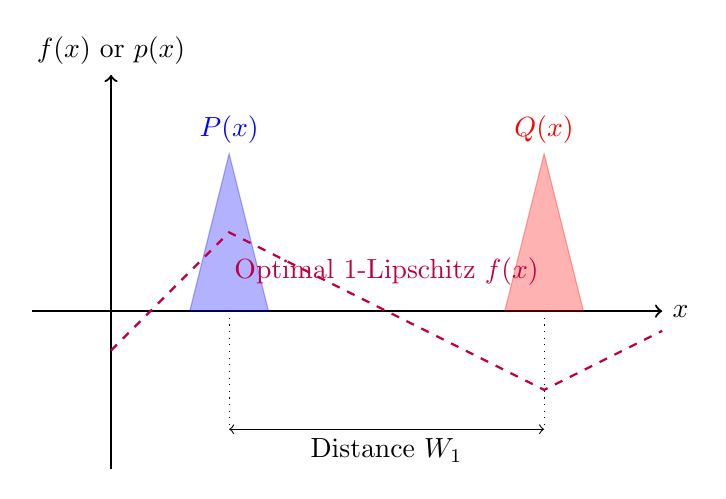
\begin{tikzpicture}
    % Axes
    \draw[->, thick] (-1, 0) -- (7, 0) node[right] {$x$};
    \draw[->, thick] (0, -2) -- (0, 3) node[above] {$f(x)$ or $p(x)$};
    
    % Distributions
    \filldraw[blue, opacity=0.3] (1,0) -- (1.5, 2) -- (2,0) -- cycle;
    \node[blue] at (1.5, 2.3) {$P(x)$};
    
    \filldraw[red, opacity=0.3] (5,0) -- (5.5, 2) -- (6,0) -- cycle;
    \node[red] at (5.5, 2.3) {$Q(x)$};
    
    % Lipschitz Function
    \draw[thick, dashed, purple] (0, -0.5) -- (1.5, 1) -- (5.5, -1) -- (7, -0.25);
    \node[purple] at (3.5, 0.5) {Optimal 1-Lipschitz $f(x)$};
    
    % Annotations
    \draw[<->] (1.5, -1.5) -- (5.5, -1.5) node[midway, below] {Distance $W_1$};
    \draw[dotted] (1.5, 0) -- (1.5, -1.5);
    \draw[dotted] (5.5, 0) -- (5.5, -1.5);
\end{tikzpicture}
\caption{The Wasserstein distance finds a smooth 1-Lipschitz function $f$ that maximizes the difference in expectations between $P$ and $Q$. The slope is bounded, ensuring that as $P$ translates towards $Q$, the distance changes continuously.}
\label{fig:wasserstein_ipm}
\end{figure}

\subsubsection{Maximum Mean Discrepancy (MMD)}
Let $\mathcal{H}$ be a Reproducing Kernel Hilbert Space (RKHS) associated with a positive definite kernel $k: \mathcal{X} \times \mathcal{X} \to \mathbb{R}$. Let $\mathcal{F}_{\text{MMD}}$ be the unit ball in $\mathcal{H}$:
\begin{equation}
    \mathcal{F}_{\text{MMD}} = \{ f \in \mathcal{H} \mid \| f \|_{\mathcal{H}} \le 1 \}.
\end{equation}
The resulting IPM is the Maximum Mean Discrepancy (MMD). Unlike the Wasserstein distance, which requires solving a complex optimization problem, MMD admits a closed-form solution.

\section{Maximum Mean Discrepancy: A Closer Look}

The elegant theory of RKHS allows us to compute the MMD without explicitly searching over the function class $\mathcal{F}_{\text{MMD}}$. By the reproducing property, for any $f \in \mathcal{H}$ and $x \in \mathcal{X}$, $f(x) = \langle f, k(x, \cdot) \rangle_{\mathcal{H}}$.

\begin{theorem}[Closed-Form MMD]
\label{thm:mmd_closed_form}
The squared Maximum Mean Discrepancy between $P$ and $Q$ corresponding to the kernel $k$ can be expressed solely in terms of kernel evaluations:
\begin{equation}
    \text{MMD}^2(P, Q) = \mathbb{E}_{X, X' \sim P}[k(X, X')] - 2\mathbb{E}_{X \sim P, Y \sim Q}[k(X, Y)] + \mathbb{E}_{Y, Y' \sim Q}[k(Y, Y')],
\end{equation}
where $X, X'$ are independent draws from $P$, and $Y, Y'$ are independent draws from $Q$.
\end{theorem}

\begin{proof}
Let $\phi(x) = k(x, \cdot) \in \mathcal{H}$ be the feature map. By the reproducing property and linearity of expectation, the expected value of $f(X)$ under $P$ is:
\begin{equation*}
    \mathbb{E}_{X \sim P}[f(X)] = \mathbb{E}_{X \sim P}[\langle f, \phi(X) \rangle_{\mathcal{H}}] = \langle f, \mathbb{E}_{X \sim P}[\phi(X)] \rangle_{\mathcal{H}}.
\end{equation*}
Define the mean embedding of $P$ as $\mu_P = \mathbb{E}_{X \sim P}[\phi(X)] \in \mathcal{H}$. Similarly, $\mu_Q = \mathbb{E}_{Y \sim Q}[\phi(Y)]$.
The IPM becomes:
\begin{align*}
    \text{MMD}(P, Q) &= \sup_{\| f \|_{\mathcal{H}} \le 1} \left( \langle f, \mu_P \rangle_{\mathcal{H}} - \langle f, \mu_Q \rangle_{\mathcal{H}} \right) \\
    &= \sup_{\| f \|_{\mathcal{H}} \le 1} \langle f, \mu_P - \mu_Q \rangle_{\mathcal{H}}.
\end{align*}
By the Cauchy-Schwarz inequality, $\langle f, \mu_P - \mu_Q \rangle_{\mathcal{H}} \le \|f\|_{\mathcal{H}} \| \mu_P - \mu_Q \|_{\mathcal{H}} \le \| \mu_P - \mu_Q \|_{\mathcal{H}}$. The supremum is achieved when $f$ is aligned with $(\mu_P - \mu_Q) / \| \mu_P - \mu_Q \|_{\mathcal{H}}$, giving:
\begin{equation*}
    \text{MMD}(P, Q) = \| \mu_P - \mu_Q \|_{\mathcal{H}}.
\end{equation*}
Squaring this norm yields:
\begin{align*}
    \text{MMD}^2(P, Q) &= \| \mu_P - \mu_Q \|_{\mathcal{H}}^2 \\
    &= \langle \mu_P - \mu_Q, \mu_P - \mu_Q \rangle_{\mathcal{H}} \\
    &= \langle \mu_P, \mu_P \rangle_{\mathcal{H}} - 2 \langle \mu_P, \mu_Q \rangle_{\mathcal{H}} + \langle \mu_Q, \mu_Q \rangle_{\mathcal{H}}.
\end{align*}
Expanding the inner products of the mean embeddings recovers the theorem:
\begin{align*}
    \langle \mu_P, \mu_P \rangle_{\mathcal{H}} &= \langle \mathbb{E}_{X}[\phi(X)], \mathbb{E}_{X'}[\phi(X')] \rangle_{\mathcal{H}} = \mathbb{E}_{X, X'}[\langle \phi(X), \phi(X') \rangle_{\mathcal{H}}] = \mathbb{E}_{X, X'}[k(X, X')],
\end{align*}
and similarly for the other terms. This completes the proof.
\end{proof}

\begin{figure}[htbp]
\centering
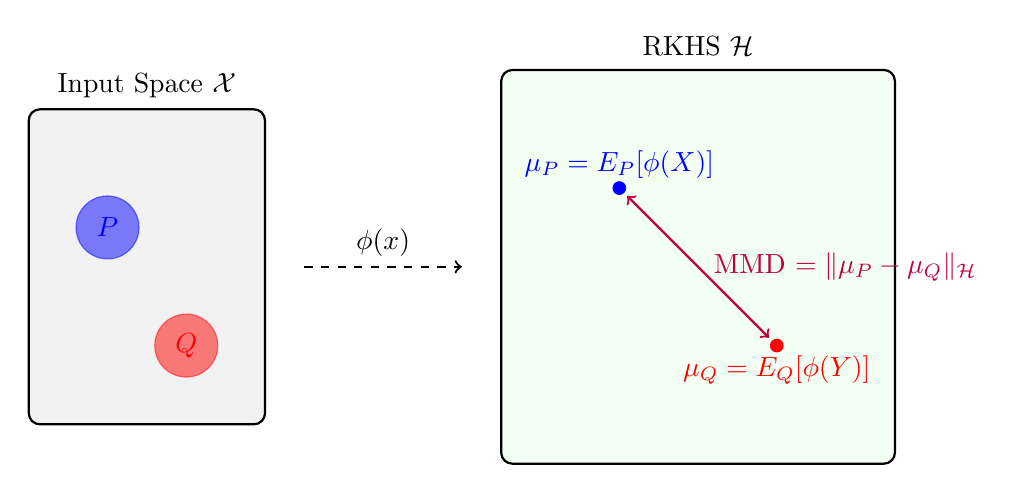
\begin{tikzpicture}
    % Input Space
    \draw[thick, fill=gray!10, rounded corners] (-4, -2) rectangle (-1, 2);
    \node at (-2.5, 2.3) {Input Space $\mathcal{X}$};
    
    \filldraw[blue, opacity=0.5] (-3, 0.5) circle (0.4);
    \node[blue] at (-3, 0.5) {$P$};
    
    \filldraw[red, opacity=0.5] (-2, -1) circle (0.4);
    \node[red] at (-2, -1) {$Q$};

    % Mapping arrow
    \draw[->, thick, dashed] (-0.5, 0) -- (1.5, 0) node[midway, above] {$\phi(x)$};

    % RKHS
    \draw[thick, fill=green!5, rounded corners] (2, -2.5) rectangle (7, 2.5);
    \node at (4.5, 2.8) {RKHS $\mathcal{H}$};

    \filldraw[blue] (3.5, 1) circle (0.08) node[above] {$\mu_P = \mathbb{E}_P[\phi(X)]$};
    \filldraw[red] (5.5, -1) circle (0.08) node[below] {$\mu_Q = \mathbb{E}_Q[\phi(Y)]$};

    \draw[<->, thick, purple] (3.6, 0.9) -- (5.4, -0.9) node[midway, right=2pt] {MMD $= \| \mu_P - \mu_Q \|_{\mathcal{H}}$};

\end{tikzpicture}
\caption{MMD conceptually maps distributions $P$ and $Q$ into a Reproducing Kernel Hilbert Space via feature map $\phi$. The MMD is simply the distance between their mean embeddings $\mu_P$ and $\mu_Q$ in this high-dimensional space.}
\label{fig:mmd_rkhs}
\end{figure}

\subsection{Numerical Example: Empirical MMD}

Suppose we have two finite samples $X = \{x_1, x_2\} \sim P$ and $Y = \{y_1, y_2\} \sim Q$, with $x_1 = 0, x_2 = 1$ and $y_1 = 2, y_2 = 3$.
We choose a linear kernel $k(a, b) = a \cdot b$.

The empirical squared MMD is an unbiased estimator given by:
\begin{equation}
    \widehat{\text{MMD}}^2 = \frac{1}{n(n-1)} \sum_{i \neq j} k(x_i, x_j) + \frac{1}{m(m-1)} \sum_{i \neq j} k(y_i, y_j) - \frac{2}{nm} \sum_{i=1}^n \sum_{j=1}^m k(x_i, y_j).
\end{equation}

For $X = \{0, 1\}$, $x_1 x_2 + x_2 x_1 = 0 + 0 = 0$. So the first term is $0 / 2 = 0$.
For $Y = \{2, 3\}$, $y_1 y_2 + y_2 y_1 = 6 + 6 = 12$. The second term is $12 / 2 = 6$.
For the cross-term, the sum is $(0 \cdot 2) + (0 \cdot 3) + (1 \cdot 2) + (1 \cdot 3) = 0 + 0 + 2 + 3 = 5$. The third term is $-2 \cdot (5 / 4) = -2.5$.

Thus, $\widehat{\text{MMD}}^2 = 0 + 6 - 2.5 = 3.5$. 
The distance reflects the shift in the mean between the two samples, cleanly captured by the linear kernel (where the mean embedding is just the standard mean). With more complex kernels (like Gaussian RBF), MMD can detect differences in variance and higher moments.

\begin{horizon}
While traditional IPMs like MMD and Wasserstein distance require carefully crafted function classes (RKHS balls, Lipschitz continuous functions), modern generative modeling increasingly relies on \textit{Neural IPMs}. In this setting, the discriminator class $\mathcal{F}$ is explicitly parameterized by a deep neural network, $\mathcal{F}_\Theta = \{ f_\theta \mid \theta \in \Theta \}$. 

It is conjectured that when $\mathcal{F}_\Theta$ is appropriately overparameterized, it possesses sufficient capacity to approximate the true Wasserstein-1 distance (provided strict Lipschitz constraints are enforced via spectral normalization or gradient penalties). However, an open question remains regarding the statistical sample complexity of Neural IPMs in extremely high dimensions. Theoretical bounds for traditional IPMs depend heavily on the Rademacher complexity of $\mathcal{F}$, which is notoriously loose for neural networks. 

Future work might show precisely how the implicit bias of gradient descent on the discriminator network constrains its effective capacity, potentially yielding much tighter generalization bounds than those derived from worst-case bounds on the entire neural network hypothesis class. Closing this gap would provide a rigorous foundation for why highly parameterized GANs do not immediately collapse to empirically memorizing the training data, and would firmly link neural empirical distributions with true underlying data manifolds.
\end{horizon}

\section{Summary}
In this chapter, we stepped away from density-based divergences and introduced Integral Probability Metrics (IPMs). By redefining distance as the maximum discrepancy over a class of test functions, IPMs provide continuous, well-behaved metrics even when distributions lack overlapping support. We proved that symmetric function classes yield a simplified IPM definition, and demonstrated that constraining the function class yields classical distances: 1-Lipschitz functions yield the Wasserstein-1 distance, while the unit ball of an RKHS yields the Maximum Mean Discrepancy (MMD). Crucially, MMD admits a closed-form solution via kernel embeddings, bypassing complex optimization.

\section{Exercises}

\begin{enumerate}
    \item \textbf{Total Variation as an IPM:} Let $\mathcal{F}_{\text{TV}}$ be the set of all measurable functions $f$ such that $\sup_x |f(x)| \le 1$. Show that the IPM induced by $\mathcal{F}_{\text{TV}}$ is equal to $\sup_{A \in \Sigma} |P(A) - Q(A)|$, up to a constant scalar factor. 
    \item \textbf{MMD with a Linear Kernel:} Prove that if the kernel is $k(x, y) = x^\top y$, the Maximum Mean Discrepancy $\text{MMD}(P, Q)$ reduces exactly to the Euclidean distance between the expected values (means) of the two distributions, $\| \mathbb{E}[X] - \mathbb{E}[Y] \|_2$.
    \item \textbf{Translational Invariance:} Let $P$ and $Q$ be distributions on $\mathbb{R}^d$. Let $P_c$ and $Q_c$ be the identical distributions shifted by a constant vector $c \in \mathbb{R}^d$. Prove that the Wasserstein-1 distance is translationally invariant: $W_1(P, Q) = W_1(P_c, Q_c)$.
    \item \textbf{Discriminator Optimization:} In the context of a Neural IPM, suppose $\mathcal{F}$ is parametrized by $f_\theta$. Formulate the exact loss function $\mathcal{L}(\theta)$ you would maximize to estimate the IPM between a fixed dataset $X \sim P$ and a generator producing $Y \sim Q$. How does this compare to the standard GAN discriminator loss?
\end{enumerate}

% TODO-CITE: Ensure all named results are cited.
